\documentclass[12pt]{article}
\usepackage{amsmath}
\usepackage{kotex}
\usepackage{graphicx}
\usepackage{hyperref}
\title{Assignment01}
\author{20124602 이승준}
\date{Sep.21.2018}
\begin{document}
  \maketitle
  \section[시작]{git이란?}
  	\ Git이란 오픈 소프트웨어코드 저장소의 대표적인 하나이며, git덕분에 오픈소스 업계가 큰 발전을 이루었다고 하는것은 과언이 아니다. git의 작업서버의 전체 기록과 각 기록을 추적할 수 있는 정보를 포함하고 있어서, 프로그래머가 수정하기전의 코드를 쉽게 열람이 가능하고, 이를 개인 컴퓨터에 간단한 명령어를 통해 카피 할 수 있다. github를 통하여 git으로 사람들이 공유하고있는 코드를 실체화 할 수 있다.
  	
  	다음 링크를 통하여 git을 손쉽게 설치할 수 있다.
  	
    \href{https://git-scm.com/download/win}{git 다운로드 페이지주소}
  \section{github 사용하기}
  \ git을 사용하기 위해선 우선 자신만의 github가 필요하다.
  	 \href{https://git-scm.com/download/win}{github 페이지}
  	가입은 간단하게 자신이 사용하고 있는 이메일 주소만 입력하면 가입이 완성이 될것이다.
  %	\centering
  % 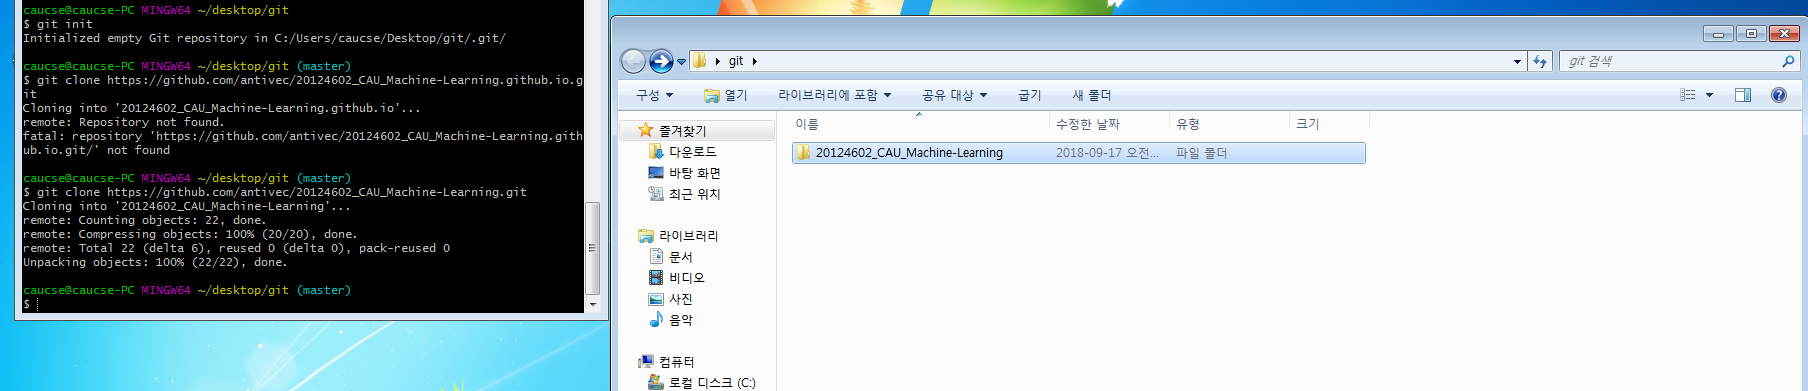
\includegraphics[width=\textheight]{git01}
  %	\href{https://github.com/antivec/20124602_CAU_Machine-Learning}{github 주소}
  % This is a comment; it will not be shown in the final output.
  % The following shows a little of the typesetting power of LaTeX:

\end{document}
	
  $ pdflatex assignment01.tex